%
% File acl2017.tex
%

\documentclass[11pt,a4paper]{article}
\usepackage[hyperref]{acl2017}
\usepackage{times}
\usepackage{url}
\usepackage{latexsym}
\usepackage{amsmath}
\usepackage{breqn}
\usepackage{pgfplotstable}
\usepackage{algorithm2e}
\usepackage{hhline}
\usepackage{multirow}
\usepackage[font=small]{caption}
\usepackage{subcaption}
\usepackage{color}
\usepackage{float}
\usepackage{lipsum,adjustbox}
\usepackage{tikz}
\usepackage{tikz-dependency}
\usepackage{enumitem}
\usepackage{xr}
\externaldocument{acl2017_supp}
\usetikzlibrary{shapes,fit,calc,er,positioning,intersections,decorations.shapes,mindmap,trees}
\tikzset{decorate sep/.style 2 args={decorate,decoration={shape backgrounds,shape=circle,
      shape size=#1,shape sep=#2}}}
\newcommand{\oa}[1]{\footnote{\color{red} #1}}
\newcommand{\daniel}[1]{\footnote{\color{blue} #1}}
\newcommand{\com}[1]{}
\newcommand{\parser}[1]{TUPA\textsubscript{#1}}
\newcommand{\secref}[1]{Section~\ref{#1}}
\newcommand{\figref}[1]{Figure~\ref{#1}}
\newcommand{\tabref}[1]{Table~\ref{#1}}
\DeclareMathOperator*{\argmin}{argmin}
\DeclareMathOperator*{\argmax}{argmax}
\SetKwRepeat{Do}{do}{while}

\hyphenation{SemEval}
\hyphenation{PARSEVAL}
\hyphenation{DAGParser}
\hyphenation{TurboSemanticParser}
\hyphenation{MaltParser}

\def\linkspace#1#2{\leavevmode
\def\tmp##1{\nolinebreak[2]\href{#1}{\hbox{##1}}}%
\xlinkspace#2 \relax}

\def\xlinkspace#1 #2{%
 \ifx\relax#2%
 \xlinkdash#1-\relax
 \else
 \xlinkdash#1 -\relax
 \expandafter\xlinkspace\expandafter#2%
 \fi}

\def\xlinkdash#1-#2{%
 \ifx\relax#2%
 \tmp{#1}%
 \else
 \tmp{#1-}%
 \expandafter\xlinkdash\expandafter#2%
 \fi}

%\aclfinalcopy % Uncomment this line for the final submission
%\def\aclpaperid{193} %  Enter the acl Paper ID here

%\setlength\titlebox{5cm}
% You can expand the titlebox if you need extra space
% to show all the authors. Please do not make the titlebox
% smaller than 5cm (the original size); we will check this
% in the camera-ready version and ask you to change it back.

\title{Broad-Coverage Transition-Based UCCA Parsing}

\author{Daniel Hershcovich$^{1,2}$ \And Omri Abend$^2$ \And Ari Rappoport$^2$ \\
  $^1$Edmond and Lily Safra Center for Brain Sciences, Hebrew University of Jerusalem \\
  $^2$School of Computer Science and Engineering, Hebrew University of Jerusalem \\
  \texttt{\{danielh,oabend,arir\}@cs.huji.ac.il}
}

\date{}

\begin{document}
\maketitle

%%%%%%%%%%%%%%%%%%%%%%%%%%%%%%%%%%%%%%%%%%%%%%%%%%%%%%%%%%%%%%%
%%%%%%%%%%%%%%%%%     Abstract     %%%%%%%%%%%%%%%%%%%%%%%%%%%%
%%%%%%%%%%%%%%%%%%%%%%%%%%%%%%%%%%%%%%%%%%%%%%%%%%%%%%%%%%%%%%%
\begin{abstract}
  We present the first parser for UCCA, a
  cross-linguistically applicable framework for semantic
  representation, which builds on extensive
  typological work, and supports rapid annotation.
  UCCA poses a challenge for existing parsing techniques,
  as it exhibits reentrancy (resulting in DAG structures),
  discontinuous structures and non-terminal nodes corresponding
  to complex semantic units. To our knowledge, the conjunction
  of these formal properties is not supported by any existing parser.
  Our transition-based parser, which uses a novel transition set
  and features based on bidirectional LSTMs,
  has value not just for UCCA parsing:
  its ability to handle more general graph structures will inform
  the development of parsers for other semantic DAG structures, 
  and in languages that frequently use discontinuous structures.
\end{abstract}


%%%%%%%%%%%%%%%%%%%%%%%%%%%%%%%%%%%%%%%%%%%%%%%%%%%%%%%%%%%%%%%
\section{Introduction}\label{sec:introduction}

Universal Conceptual Cognitive Annotation \cite[UCCA,][]{abend2013universal}
is a cross-linguistically applicable semantic representation scheme,
building on the established Basic Linguistic Theory typological framework
\cite{Dixon:10b,Dixon:10a,Dixon:12}, and Cognitive
Linguistics literature \cite{croft2004cognitive}.
It has demonstrated applicability to multiple languages, including
English, French, German and Czech, support for rapid annotation,
and stability under translation \cite{sulem2015conceptual}.
The scheme has proven useful for machine translation evaluation \cite{birch2016hume}.
UCCA differs from syntactic
schemes in terms of content and formal structure.
It exhibits reentrancy, discontinuous nodes and non-terminals,
which no single existing parser supports.
Lacking a parser, UCCA's applicability has been so far limited,
a gap this work addresses.

We present the first UCCA parser, \parser{}
(Transition-based UCCA Parser),
building on recent advances in discontinuous constituency
and dependency graph parsing, and further introducing novel transitions and features for UCCA.
Transition-based techniques are a natural
starting point for UCCA parsing, given the conceptual similarity of
UCCA's distinctions, centered around predicate-argument structures, to distinctions expressed
by dependency schemes, and the achievements of transition-based methods in dependency parsing
\cite{dyer2015transition,andor2016globally,kiperwasser2016simple}.
We are further motivated by the strength of transition-based methods
in related tasks, including dependency graph parsing
\cite{sagae2008shift,ribeyre-villemontedelaclergerie-seddah:2014:SemEval,tokgoz2015transition},
constituency parsing \cite{sagae2005classifier,zhang2009transition,zhu2013fast,maier2015discontinuous,maier-lichte:2016:DiscoNLP},
AMR parsing \cite{wang-xue-pradhan:2015:ACL-IJCNLP,wang2015transition,wang-EtAl:2016:SemEval,dipendra2016neural,goodman2016noise,zhou2016amr,damonte-17}
and CCG parsing \cite{zhang2011shift,ambati2015incremental,ambati-deoskar-steedman:2016:N16-1}.

We evaluate \parser{} on the English UCCA corpora, including in-domain and out-of-domain settings.
To assess the ability of existing
parsers to tackle the task, we develop a conversion procedure
from UCCA to bilexical graphs and trees.
Results show superior accuracy for \parser{}, demonstrating the effectiveness of
the presented approach.\footnote{Our code will be made freely available upon publication.}

The rest of the paper is structured as follows:
\secref{sec:ucca} describes UCCA in more detail.
\secref{sec:parser} introduces \parser{}.
\secref{sec:exp_setup} discusses the data and experimental setup.
\secref{sec:results} presents the experimental results.
\secref{sec:related_work} summarizes related work, and
\secref{sec:conclusion} concludes the paper.




%%%%%%%%%%%%%%%%%%%%%%%%%%%%%%%%%%%%%%%%%%%%%%%%%%%%%%%%%%%%%%%
\section{The UCCA Scheme}\label{sec:ucca}

UCCA graphs are labeled, directed acyclic graphs (DAGs),
whose leaves correspond to the tokens of
the text. A node (or {\it unit}) corresponds to a terminal or
to several sub-units (not necessarily contiguous) viewed as a
single entity according to semantic or cognitive considerations.
Edges bear a category, indicating the role of the sub-unit in the parent relation.
\figref{fig:examples} presents a few examples.

UCCA is a multi-layered representation, where each layer corresponds
to a ``module'' of semantic distinctions.
UCCA's \textit{foundational layer}, targeted in this paper, covers the predicate-argument
structure evoked by predicates of all grammatical categories
(verbal, nominal, adjectival and others), the inter-relations between them,
and other major linguistic phenomena such as coordination and multi-word expressions.
The layer's basic notion is the \textit{scene}, describing a movement, action or state.
Each scene contains one main relation (marked as either a Process or a State),
as well as one or more Participants.
For example, the sentence ``After graduation, John moved to Paris'' (\figref{fig:graduation})
contains two scenes, whose main relations are ``graduation'' and ``moved''.
``John'' is a Participant in both scenes, while ``Paris'' only in the latter.
Further categories account for inter-scene relations and the internal structure of
complex arguments and relations (e.g. coordination, multi-word expressions and modification).

One incoming edge for each non-root node is marked as \textit{primary},
and the rest (mostly used for implicit relations and arguments) as \textit{remote} edges,
a distinction made by the annotator.
The primary edges thus form a tree structure, whereas the remote edges enable reentrancy,
forming a DAG.

\begin{figure}[t]
  \begin{subfigure}{.9\columnwidth}
  \parbox{.05\columnwidth}{\caption{}\label{fig:graduation}}
  \parbox{.8\columnwidth}{
  \scalebox{.9}{
  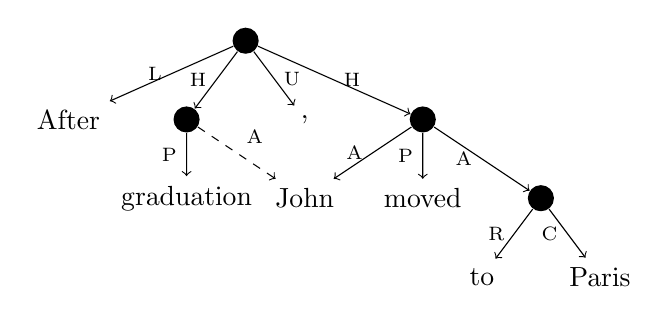
\begin{tikzpicture}[level distance=10mm, ->,
      every circle node/.append style={fill=black}]
    \node (ROOT) [circle] {}
      child {node (After) {After} edge from parent node[left] {\scriptsize L}}
      child {node (graduation) [circle] {}
      {
        child {node {graduation} edge from parent node[left] {\scriptsize P}}
      } edge from parent node[left] {\scriptsize H} }
      child {node {,} edge from parent node[right] {\scriptsize U}}
      child {node (moved) [circle] {}
      {
        child {node (John) {John} edge from parent node[left] {\scriptsize A}}
        child {node {moved} edge from parent node[left] {\scriptsize P}}
        child {node [circle] {}
        {
          child {node {to} edge from parent node[left] {\scriptsize R}}
          child {node {Paris} edge from parent node[left] {\scriptsize C}}
        } edge from parent node[left] {\scriptsize A} }
      } edge from parent node[right] {\scriptsize H} }
      ;
    \draw[dashed,->] (graduation) to node [auto] {\scriptsize A} (John);
  \end{tikzpicture}
  }}
  \end{subfigure}
  \begin{subfigure}{.9\columnwidth}
  \vspace{-2cm}
  \parbox{.05\columnwidth}{\caption{}\label{fig:gave}}
  \parbox{.75\columnwidth}{\hspace{1cm}
  \scalebox{.9}{
  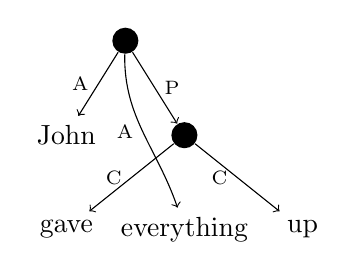
\begin{tikzpicture}[level distance=12mm, ->,
      every node/.append style={midway},
      every circle node/.append style={fill=black}]
    \node (ROOT) [circle] {}
      child {node {John} edge from parent node[left] {\scriptsize A}}
      child {node [circle] {}
      {
      	child {node {gave} edge from parent node[left] {\scriptsize C}}
      	child {node (everything) {everything} edge from parent[white]}
      	child {node {up} edge from parent node[left] {\scriptsize C}}
      } edge from parent node[right] {\scriptsize P} }
      ;
    \draw[bend right,->] (ROOT) to[out=-20, in=180] node [left] {\scriptsize A} (everything);
  \end{tikzpicture}
  }}
  \parbox{.1\columnwidth}{
  \vspace{2cm}
  \begin{adjustbox}{width=.3\columnwidth,margin=1pt,frame}
  \begin{tabular}{ll}
  P & process \\
  A & participant \\
  H & linked scene \\
  C & center \\
  R & relator \\
  N & connector \\
  L & scene linker \\
  U & punctuation \\
  F & function unit
  \end{tabular}
  \end{adjustbox}
  }
  \end{subfigure}
  \begin{subfigure}{.9\columnwidth}
  \vspace{-1cm}
  \parbox{.05\columnwidth}{\caption{}\label{fig:home}}
  \parbox{.65\columnwidth}{
  \scalebox{.9}{
  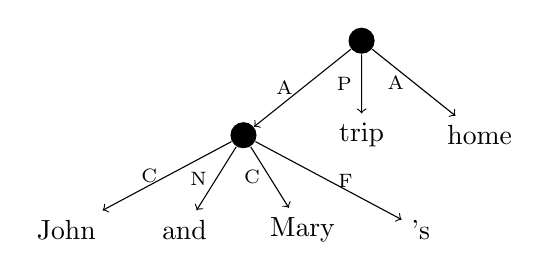
\begin{tikzpicture}[level distance=12mm, ->,
      every node/.append style={midway},
      every circle node/.append style={fill=black}]
    \node (ROOT) [circle] {}
      child {node [circle] {}
      {
        child {node {John} edge from parent node[left] {\scriptsize C}}
        child {node {and} edge from parent node[left] {\scriptsize N}}
        child {node {Mary} edge from parent node[left] {\scriptsize C}}
        child {node {'s} edge from parent node[right] {\scriptsize F}}
      } edge from parent node[left] {\scriptsize A} }
      child {node {trip} edge from parent node[left] {\scriptsize P}}
      child {node {home} edge from parent node[left] {\scriptsize A}}
      ;
  \end{tikzpicture}
  }}
  \end{subfigure}
  \caption{\label{fig:examples}
    UCCA structures demonstrating three structural properties exhibited by
    the scheme.
    (\subref{fig:graduation}) includes a remote edge (dashed),
    resulting in ``John'' having two parents.
    (\subref{fig:gave}) includes a discontinuous unit (``gave ... up'').
    (\subref{fig:home}) includes a coordination construction (``John and Mary'').
    Pre-terminal nodes are omitted for brevity.
    Right: legend of edge labels.
  }
\end{figure}

While parsing technology in general, and transition-based parsing in particular,
is well-established for syntactic parsing, UCCA
has several distinct properties
that distinguish it from syntactic representations,
mostly UCCA's tendency to abstract away from syntactic detail that do not
affect argument structure.
%.\footnote{As essentially any change in form results
%in some change in meaning, it would be more precise to say that
%UCCA's foundational layer abstracts away from syntactic variation
%not affecting argument structure and other aspects of meaning it covers.}
For instance, consider the following examples where the concept of a scene
has a different rationale from the syntactic concept of a clause.
First, non-verbal predicates in UCCA are represented like verbal ones,
such as when they appear in copula clauses or noun phrases. Indeed,
in \figref{fig:graduation}, ``graduation'' and ``moved'' are considered separate events,
despite appearing in the same clause. 
Second, in the same example, ``John'' is marked as a (remote) Participant
in the graduation scene, despite not being overtly marked.
Third, consider the possessive construction in \figref{fig:home}.
While in UCCA ``trip'' evokes a scene in which ``John and Mary'' is
a Participant, a syntactic scheme would analyze this phrase similarly to ``John and Mary's children''.

These abstractions are not structurally explicit by their nature
(e.g., ``after graduation'' is formally very similar to ``after 2pm'',
which does not evoke a scene), suggesting that a UCCA parser, and more generally semantic parsers,
are required to produce different types of generalizations than those required by their syntactic counterparts.
\secref{sec:related_work} discusses UCCA in the context of other semantic schemes,
such as AMR \cite{banarescu2013abstract}.

%These properties distinguish UCCA from syntactic schemes that already have
%established parsing techonology, and will likely require different techniques.

Alongside recent progress in dependency parsing into projective trees,
there is increasing interest in parsing into 
representations with more general structural properties  (see \secref{sec:related_work}).
One such property is \textit{reentrancy},
namely the sharing of semantic units between predicates.
For instance, in \figref{fig:graduation},
``John'' is an argument of both ``graduation''
and ``moved'', yielding a DAG rather than a tree.
A second property is \textit{discontinuity},
as in \figref{fig:gave}, where ``gave up'' forms a discontinuous semantic unit.
Discontinuities are pervasive, e.g.,  with multi-word
expressions \cite{schneider2014discriminative}.
Finally, unlike most dependency schemes, UCCA uses \textit{non-terminal nodes}
to represent units comprising more than one word.
The use of non-terminal nodes is motivated by constructions with no clear head, including
coordination structures (e.g., ``John and Mary'' in \figref{fig:home}),
some multi-word expressions (e.g., ``The Haves and the \textit{Have Nots}''),
and prepositional phrases (either the preposition or the head noun can serve as the constituent's head).
To our knowledge, no existing parser supports all structural properties required for UCCA
parsing.



%%%%%%%%%%%%%%%%%%%%%%%%%%%%%%%%%%%%%%%%%%%%%%%%%%%%%%%%%%%%%%%
\section{Transition-based UCCA Parsing}\label{sec:parser}

We now turn to presenting \parser{}.
Building on previous work on parsing reentrancies, discontinuities and non-terminal nodes,
we define an extended set of transitions and features that supports the conjunction of
these properties.

Transition-based parsers \cite{Nivre03anefficient} scan the text from start to end,
and create the parse incrementally by applying a \textit{transition}
at each step to the parser state,
defined using three data structures: a buffer $B$ of tokens and nodes to be processed,
a stack $S$ of nodes currently being processed,
and a graph $G=(V,E,\ell)$ of constructed nodes and edges,
where $V$ is the set of \emph{nodes}, $E$ is the set of \emph{edges},
and $\ell : E \to L$ is the \emph{label} function, $L$ being the set of possible labels.
Some states are marked as \textit{terminal}, meaning that $G$ is the final output.
A classifier is used at each step to select the next transition based on features
encoding the parser's current state.
During training, an oracle creates training instances for the classifier,
based on gold-standard annotations.


\begin{figure*}
\begin{adjustbox}{width=\textwidth,margin=3pt,frame}
\begin{tabular}{llll|l|llllc|c}
\multicolumn{4}{c|}{\textbf{\small Before Transition}} & \textbf{\small Transition} & \multicolumn{5}{c|}{\textbf{\small After Transition}} & \textbf{\small Condition} \\
\textbf{\footnotesize Stack} & \textbf{\footnotesize Buffer} & \textbf{\footnotesize Nodes} & \textbf{\footnotesize Edges} & & \textbf{\footnotesize Stack} & \textbf{\footnotesize Buffer} & \textbf{\footnotesize Nodes} & \textbf{\footnotesize Edges} & \textbf{\footnotesize Terminal?} & \\
$S$ & $x \;|\; B$ & $V$ & $E$ & \textsc{Shift} & $S \;|\; x$ & $B$ & $V$ & $E$ & $-$ & \\
$S \;|\; x$ & $B$ & $V$ & $E$ & \textsc{Reduce} & $S$ & $B$ & $V$ & $E$ & $-$ & \\
$S \;|\; x$ & $B$ & $V$ & $E$ & \textsc{Node$_X$} & $S \;|\; x$ & $y \;|\; B$ & $V \cup \{ y \}$ & $E \cup \{ (y,x)_X \}$ & $-$ &
$x \neq \mathrm{root}$ \\
$S \;|\; y,x$ & $B$ & $V$ & $E$ & \textsc{Left-Edge$_X$} & $S \;|\; y,x$ & $B$ & $V$ & $E \cup \{ (x,y)_X \}$ & $-$ &
\multirow{4}{50pt}{\vspace{-5mm}\[\left\{\begin{array}{l}
x \not\in w_{1:n},\\
y \neq \mathrm{root},\\
y \not\leadsto_G x
\end{array}\right.\]} \\
$S \;|\; x,y$ & $B$ & $V$ & $E$ & \textsc{Right-Edge$_X$} & $S \;|\; x,y$ & $B$ & $V$ & $E \cup \{ (x,y)_X \}$ & $-$ & \\
$S \;|\; y,x$ & $B$ & $V$ & $E$ & \textsc{Left-Remote$_X$} & $S \;|\; y,x$ & $B$ & $V$ & $E \cup \{ (x,y)_X^* \}$ & $-$ & \\
$S \;|\; x,y$ & $B$ & $V$ & $E$ & \textsc{Right-Remote$_X$} & $S \;|\; x,y$ & $B$ & $V$ & $E \cup \{ (x,y)_X^* \}$ & $-$ & \\
$S \;|\; x,y$ & $B$ & $V$ & $E$ & \textsc{Swap} & $S \;|\; y$ & $x \;|\; B$ & $V$ & $E$ & $-$ &
$\mathrm{i}(x) < \mathrm{i}(y)$ \\
$[\mathrm{root}]$ & $\emptyset$ & $V$ & $E$ & \textsc{Finish} & $\emptyset$ & $\emptyset$ & $V$ & $E$ & $+$ & \\
\end{tabular}
\end{adjustbox}
\caption{\label{fig:transitions}
  The transition set of \parser{}. %Following standard practice,
  We write the stack with its top to the right and the buffer with its head to the left.
  $(\cdot,\cdot)_X$ denotes a primary $X$-labeled edge, and $(\cdot,\cdot)_X^*$ a remote $X$-labeled edge.
  $\mathrm{i}(x)$ is a running index for the created nodes.
  In addition to the specified conditions,
  the prospective child in an \textsc{Edge} transition must not already have a primary parent.
}
\end{figure*}

\paragraph{Transition Set.}
Given a sequence of tokens $w_1, \ldots, w_n$, we predict a UCCA graph $G$ over the sequence.
Parsing starts with a single node on the stack (an artificial root node), and the input tokens
in the buffer. The set of transitions is given in \figref{fig:transitions}.
In addition to the standard \textsc{Shift} and \textsc{Reduce} operations, 
we follow previous work in transition-based constituency parsing \cite{sagae2005classifier},
adding the \textsc{Node} transition for creating new non-terminal nodes.
\textsc{Node$_X$} creates a new node on the buffer as a parent of the first element on the stack, with an $X$-labeled edge.

\textsc{Left-Edge$_X$} and \textsc{Right-Edge$_X$} create a new primary $X$-labeled edge between the first two elements on the stack, where the parent is the left or the right node, respectively.
As a UCCA node may only have one incoming primary edge,
\textsc{Edge} transitions are disallowed if the child node already
has an incoming primary edge.
\textsc{Left-Remote$_X$} and \textsc{Right-Remote$_X$} do not have this restriction,
and the created edge is additionally marked as \textit{remote}.
We distinguish between these two pairs of transitions to allow the parser to create remote edges
without the possibility of producing invalid graphs.
To support the prediction of multiple parents, node and edge transitions
leave the stack unchanged, as in other work on
transition-based dependency graph parsing
\cite{sagae2008shift,ribeyre-villemontedelaclergerie-seddah:2014:SemEval,tokgoz2015transition}.
\textsc{Reduce} pops the stack, to allow removing a node
once all its edges have been created.
To handle discontinuous nodes, \textsc{Swap} pops the second
node on the stack and adds it to the top of the buffer, as with the similarly
named transition in previous work \cite{nivre2009non,maier2015discontinuous}.
Finally, \textsc{Finish} pops the root node and marks the state as terminal.

\paragraph{Classifier.}
The choice of classifier and feature representation has been shown to play an important role in
transition-based parsing \cite{chen2014fast,andor2016globally,kiperwasser2016simple}.
To investigate the impact of the type of transition classifier in UCCA parsing,
we experiment with three different models.
\begin{enumerate}[leftmargin=*]
\item
Starting with a simple and common choice \cite[e.g.,][]{maier-lichte:2016:DiscoNLP},
\textbf{\parser{Sparse}} uses a linear classifier with sparse features, trained with
the averaged structured perceptron algorithm
\cite{Coll:04} and \textsc{MinUpdate} \cite{goldberg2011learning}:
each feature requires a minimum number of updates in training
to be included in the model.\footnote{We also experimented with a linear model using
dense embedding features, but still trained with averaged structured perceptron.
It performed worse than the sparse perceptron model and was hence discarded.}
\item
Changing the model to a feedforward neural network with dense embedding features,
\textbf{\parser{MLP}}
(``multi-layer perceptron''), uses an architecture similar to that of \citet{chen2014fast},
but with two rectified linear layers
and dropout \cite{srivastava2014dropout}.
The embeddings are trained jointly with the classifier.
\item
Finally, \textbf{\parser{BiLSTM}} uses a bidirectional LSTM for feature representation,
on top of the dense embedding features,
using an architecture similar to \citet{kiperwasser2016simple}.
The BiLSTM runs on the input tokens in both forward and backward directions,
yielding a vector representation that is then concatenated with dense features representing the
parser state (e.g., existing edge labels and previous parser actions).
This representation is then fed into a feedforward network similar to \parser{MLP}.
The feedforward layers, BiLSTM and embeddings are all trained jointly.
\end{enumerate}

For all classifiers, inference is performed greedily, i.e., without beam search.
Hyperparameters are tuned on the development set (see \secref{sec:exp_setup}).

\begin{figure}[t]
	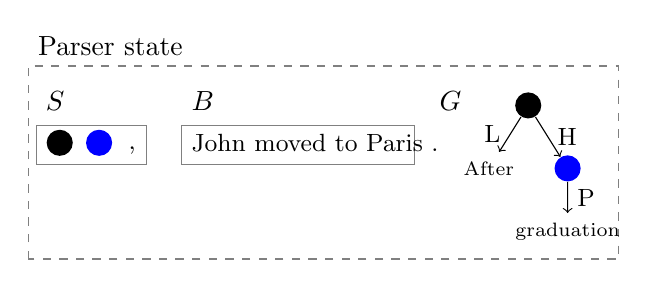
\begin{tikzpicture}[level distance=8mm, sibling distance=1cm]
	\node[anchor=west] at (0,1.5) {Parser state};
	\draw[color=gray,dashed] (0,-1.2) rectangle (7.5,1.25);
	\draw[color=gray] (.1,0) rectangle (1.5,.5);
	\node[anchor=west] at (.1,.8) {$S$};
	\node[fill=black, circle] at (.4,.275) {};
	\node[fill=blue, circle] at (.9,.275) {};
	\node[anchor=west] at (1.15,.175) {\small ,};
	\draw[color=gray] (1.95,0) rectangle (4.9,.5);
	\node[anchor=west] at (1.95,.8) {$B$};
	\node[anchor=west] at (1.95,.275) {\small John moved to Paris .};
	\node[anchor=west] at (5.1,.8) {$G$};
	\node[fill=black, circle] at (6.35,.75) {}
	  child {node  {\scriptsize After} edge from parent [->] node[left] {\small L}}
	  child {node [fill=blue, circle] {}
	  {
	    child {node {\scriptsize graduation} edge from parent [->] node[right] {\small P}}
	  } edge from parent [->] node[right] {\small H} };
	\end{tikzpicture}
	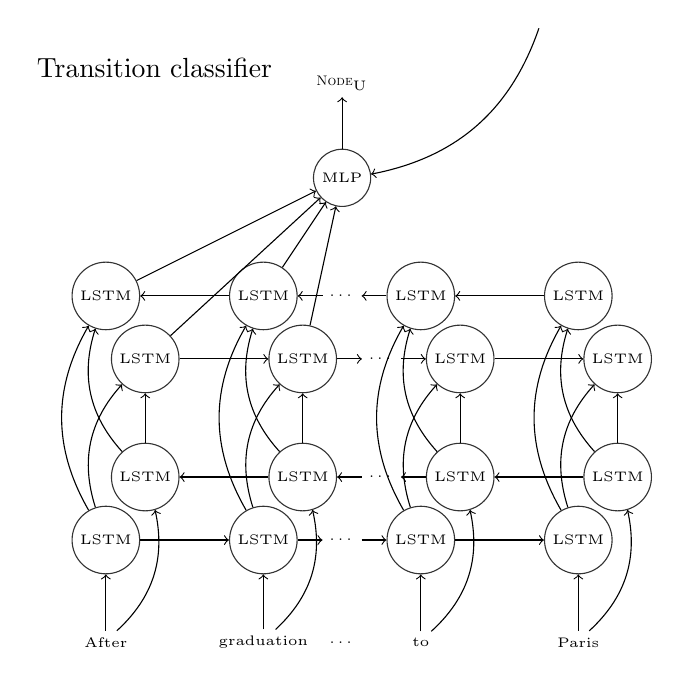
\begin{tikzpicture}[->]
	\node[anchor=west] at (0,6) {Transition classifier};
	\tiny
	\tikzstyle{main}=[circle, minimum size=7mm, draw=black!80, node distance=12mm]
	\foreach \i/\word in {1/{After},3/{graduation},5/{to},7/{Paris}} {
	    \node (x\i) at (\i,-1.3) {\word};
	    \node[main, fill=white!100] (h\i) at (\i,0) {LSTM};
        \path (x\i) edge (h\i);
	    \node[main, fill=white!100] (i\i) at (\i.5,.8) {LSTM};
        \path (x\i) edge [bend right] (i\i);
	    \node[main, fill=white!100] (l\i) at (\i.5,2.3) {LSTM};
        \path (h\i) edge [bend left] (l\i);
        \path (i\i) edge (l\i);
	    \node[main, fill=white!100] (k\i) at (\i,3.1) {LSTM};
        \path (i\i) edge [bend left] (k\i);
        \path (h\i) edge [bend left] (k\i);
	}
    \node (l4) at (4.5,2.3) {\ldots};
    \node (k4) at (4,3.1) {\ldots};
    \node (i4) at (4.5,.8) {\ldots};
    \node (h4) at (4,0) {\ldots};
    \node (x4) at (4,-1.3) {\ldots};
	\foreach \current/\next in {1/3,3/4,4/5,5/7} {
        \path (i\next) edge (i\current);
        \path (h\current) edge (h\next);
        \path (k\next) edge (k\current);
        \path (l\current) edge (l\next);
	}
    \node[main, fill=white!100] (mlp) at (4,4.6) {MLP};
	\foreach \i in {1,3} {
        \path (l\i) edge (mlp);
        \path (k\i) edge (mlp);
    }
    \coordinate (state) at (6.5,6.5);
    \path (state) edge [bend left] (mlp);
    \node (transition) at (4,5.8) {\textsc{Node}\textsubscript{U}};
    \path (mlp) edge (transition);
	\end{tikzpicture}
	\caption{Illustration of the parser model.
	Top: parser state (stack, buffer and intermediate graph).
	Bottom: \parser{BiLTSM} architecture.
	Vector representation for the input tokens is computed
	by two layers of bidirectional LSTMs.
	The vectors for specific tokens are concatenated with
	embedding and numeric features from the parser state
	(for existing edge labels, number of children, etc.),
	and fed into the MLP for selecting the next transition.}
	\label{fig:model}
\end{figure}

\paragraph{Features.}
\parser{Sparse} uses binary indicator features representing
the words, POS tags, syntactic dependency labels and
existing edge labels related to the top four stack elements and the 
next three buffer elements, in addition to their children and grandchildren in the graph.
We also use bi- and trigram features based on these values \cite{zhang2009transition,zhu2013fast},
features related to discontinuous nodes
\cite[including separating punctuation and gap type]{maier2015discontinuous},
features representing existing edges and the number of parents and children a node has,
and the past actions taken by the parser.
We also use a novel, UCCA-specific feature:
number of remote children.\footnote{See
Appendix~\ref{appendix:features} for a full list of used feature templates.}

For \parser{MLP} and \parser{BiLSTM},
we replace all indicator features by a
concatenation of the vector embeddings of all represented elements:
words, POS tags, syntactic dependency labels, edge labels, punctuation, gap type and parser actions.
These embeddings are initialized randomly.
We additionally use external word embeddings initialized with
pre-trained word2vec vectors \cite{mikolov2013efficient},\footnote{\url{
https://goo.gl/6ovEhC}} updated during training.
In addition to dropout between NN layers, we apply word dropout 
\cite{kiperwasser2016simple}: with a certain probability, the embedding for a
word is replaced with a zero vector. We do not apply word dropout to the external
word embeddings.

Finally, for all classifiers we add another real-valued feature to the input vector,
\textbf{ratio}, corresponding to the ratio between the number of terminals to number of nodes
in the graph $G$.
This novel feature serves as a regularizer for the creation of new nodes,
and should be beneficial for other transition-based constituency parsers too.

\paragraph{Training.}
For training the transition classifiers, we use a dynamic oracle \cite{goldberg2012dynamic},
i.e., an oracle that outputs a set of optimal transitions: when
applied to the current parser state, the gold
standard graph is reachable from the resulting state.
For example, the oracle would predict a \textsc{Node} transition if the stack 
has on its top a parent in the gold graph that has not been created,
but would predict a \textsc{Right-Edge} transition if the second stack
element is a parent of the
first element according to the gold graph and the edge between them has not been created.
The transition predicted by the classifier is deemed correct
and is applied to the parser state to reach the subsequent state,
if the transition is included in the set of optimal transitions.
Otherwise, a random optimal transition is applied,
and for the perceptron-based parser, the classifier's weights are updated according
to the perceptron update rule.

POS tags and syntactic dependency labels are extracted using spaCy
\cite{honnibal-johnson:2015:EMNLP}.\footnote{\url{https://spacy.io}}
We use the categorical cross-entropy objective function and optimize the
NN classifiers with the Adam optimizer \cite{kingma2014adam}.



%%%%%%%%%%%%%%%%%%%%%%%%%%%%%%%%%%%%%%%%%%%%%%%%%%%%%%%%%%%%%%%
\section{Experimental Setup}\label{sec:exp_setup}

\paragraph{Data.}
We conduct our experiments on the UCCA Wikipedia corpus (henceforth, \textit{Wiki}),
and use the English part of the UCCA \textit{Twenty Thousand Leagues Under the Sea}
English-French parallel corpus (henceforth, \textit{20K Leagues}) as
out-of-domain data.\footnote{\mbox{\url{http://cs.huji.ac.il/~oabend/ucca.html}}}
\tabref{table:data} presents some statistics for the two corpora.
We use passages of indices up to 676
of the \textit{Wiki} corpus as our training set, passages 688--808 as development set,
and passages 942--1028 as in-domain test set.
While UCCA edges can cross sentence boundaries, we adhere to the common
practice in semantic parsing and train our parsers on individual sentences,
discarding inter-relations between them (0.18\% of the edges).
We also discard linkage nodes and edges (as they often express inter-sentence
relations and are thus mostly redundant when applied at the sentence level)
as well as implicit nodes.\footnote{Appendix~\ref{appendix:extended_ucca}
further discusses linkage and implicit units.}
In the out-of-domain experiments, we apply the same parsers
(trained on the \textit{Wiki} training set) to the \textit{20K Leagues} corpus
without parameter re-tuning.


\begin{table}
\scalebox{.9}{
\begin{tabular}{l|ccc|c}
& \multicolumn{3}{c|}{Wiki} & 20K \\
& \small Train & \small Dev & \small Test & Leagues \\
\hline
\# passages & 300 & 34 & 33 & 154 \\
\# sentences & 4268 & 454 & 503 & 506 \\
\hline
\# nodes & 298,993 & 33,704 & 35,718 & 29,315 \\
\% terminal & 42.96 & 43.54 & 42.87 & 42.09 \\
\% non-term. & 58.33 & 57.60 & 58.35 & 60.01 \\
\% discont. & 0.54 & 0.53 & 0.44 & 0.81 \\
\% reentrant & 2.38 & 1.88 & 2.15 & 2.03 \\
\hline
\# edges & 287,914 & 32,460 & 34,336 & 27,749 \\
\% primary & 98.25 & 98.75 & 98.74 & 97.73 \\
\% remote & 1.75 & 1.25 & 1.26 & 2.27 \\
\hline
\multicolumn{3}{l}{\footnotesize Average per non-terminal node} \\
\# children & 1.67 & 1.68 & 1.66 & 1.61 
\end{tabular}
}
\caption{Statistics of the \textit{Wiki} and \textit{20K Leagues} UCCA corpora.
All counts exclude the root node, implicit nodes, and linkage nodes and edges.
}
\label{table:data}
\end{table}

\paragraph{Implementation.}
We use the DyNet package \cite{neubig2017dynet} for implementing the NN classifiers.
Unless otherwise noted, we use the default values provided by the package.
See Appendix~\ref{appendix:hyperparameters} for the hyperparameter values we found by tuning
on the development set.

\paragraph{Evaluation.}
We define a simple measure for comparing UCCA structures
$G_p=(V_p,E_p,\ell_p)$ and $G_g=(V_g,E_g,\ell_g)$,
the predicted and gold-standard graphs, respectively, over the same
sequence of terminals $W = \{w_1,\ldots,w_n\}$.
For an edge $e=(u,v)$ in either graph,
$u$ being the parent and $v$ the child, its yield $y(e) \subseteq W$ is the
set of terminals in $W$ that are descendants of $v$.
Define the set of \textit{mutual edges} between $G_p$ and $G_g$:

\vspace{-.6cm}

{\small
\begin{multline*}
    M(G_p,G_g) = \\
    \left\{(e_1,e_2) \in E_p \times E_g \;|\;
    y(e_1) = y(e_2) \wedge \ell_p(e_1)=\ell_g(e_2)\right\}
\end{multline*}
}

\vspace{-.6cm}

Labeled precision and recall are defined by dividing $|M(G_p,G_g)|$ by $|E_p|$ and $|E_g|$, respectively,
and F-score by taking their harmonic mean.
We report two variants of this measure: one where we consider only primary edges,
and another for remote edges (see \secref{sec:ucca}).
Performance on remote edges is of pivotal importance in this investigation,
which focuses on extending the class of graphs supported by statistical parsers.

We note that the measure collapses to the standard
PARSEVAL constituency evaluation measure if $G_p$ and $G_g$ are trees.
Punctuation is excluded from the evaluation, but not from the datasets.

\begin{figure}
\centering
\scalebox{.9}{
\begin{dependency}[theme = simple]
\begin{deptext}[column sep=.7em,ampersand replacement=\^]
After \^ graduation \^ , \^ John \^ moved \^ to \^ Paris \\
\end{deptext}
\depedge{2}{1}{L}
\depedge{2}{3}{U}
\depedge[dashed]{2}{4}{A}
\depedge{5}{4}{A}
\depedge{2}{5}{H}
\depedge{7}{6}{R}
\depedge{5}{7}{A}
\end{dependency}
}
\scalebox{.9}{
\begin{dependency}[theme = simple]
\begin{deptext}[column sep=.7em,ampersand replacement=\^]
John \^ gave \^ everything \^ up \\
\end{deptext}
\depedge{1}{2}{A}
\depedge{3}{2}{A}
\depedge{4}{2}{C}
\end{dependency}
}
\scalebox{.9}{
\begin{dependency}[theme = simple]
\begin{deptext}[column sep=.7em,ampersand replacement=\^]
John \^ and \^ Mary \^ went \^ home \\
\end{deptext}
\depedge[edge start x offset=-6pt]{1}{4}{A}
\depedge{2}{1}{N}
\depedge{3}{1}{C}
\depedge{5}{4}{A}
\end{dependency}
}
\caption{Bilexical approximation for sentences in \figref{fig:examples}.}
\label{fig:bilexical_example}
\end{figure}

\begin{table*}
\begin{tabular}{l|ccc|ccc||ccc|ccc}
& \multicolumn{6}{c||}{Wiki (in-domain)} & \multicolumn{6}{c}{20K Leagues (out-of-domain)} \\
& \multicolumn{3}{c|}{Primary} & \multicolumn{3}{c||}{Remote}
& \multicolumn{3}{c|}{Primary} & \multicolumn{3}{c}{Remote} \\
& \textbf{LP} & \textbf{LR} & \textbf{LF} & \textbf{LP} & \textbf{LR} & \textbf{LF}
& \textbf{LP} & \textbf{LR} & \textbf{LF} & \textbf{LP} & \textbf{LR} & \textbf{LF} \\
\hline
\parser{Sparse}
& 64.5 & 63.7 & 64.1 & 19.8 & 13.4 & 16
& 59.6 & 59.9 & 59.8 & 22.2 & 7.7 & 11.5 \\
%\parser{Dense} 
%& 59.1 & 58.9 & 59 & 17.4 & 12.4 & 14.5
%& 57.0 & 57.9 & 57.4 & 10.8 & 4.2 & 6.0 \\
\parser{MLP}
& 65.2 & 64.6 & 64.9 & 23.7 & 13.2 & 16.9
& 62.3 & 62.6 & 62.5 & 20.9 & 6.3 & 9.7 \\
\parser{BiLSTM}
& 74.4 & 72.7 & \textbf{73.5} & 47.4 & 51.6 & \textbf{49.4}
& 68.7 & 68.5 & \textbf{68.6} & 38.6 & 18.8 & \textbf{25.3} \\
\hline
\multicolumn{8}{l}{\rule{0pt}{2ex} \footnotesize
Bilexical Approximation (Dependency DAG Parsers)} \\
\small Upper Bound
%& \small 94.5 & \small 87.7 & \small 91 & \small 77.3 & \small 46.8 & \small 58.3
%& \small 94.8 & \small 88 & \small 91.3 & \small 66.3 & \small 32.3 & \small 43.4 \\
& & & \small 91 & & & \small 58.3
& & & \small 91.3 & & & \small 43.4 \\
DAGParser
& 61.8 & 55.8 & 58.6 & 9.5 & 0.5 & 1
& 56.4 & 50.6 & 53.4 & -- & 0 & 0 \\
TurboParser
& 57.7 & 46 & 51.2 & 77.8 & 1.8 & 3.7
& 50.3 & 37.7 & 43.1 & 100 & 0.4 & 0.8 \\
\hline
\multicolumn{8}{l}{\rule{0pt}{2ex} \footnotesize
Tree Approximation (Constituency Tree Parser)} \\
\small Upper Bound
%& \small 100 & \small 100 & \small 100 & & &
%& \small 100 & \small 100 & \small 100 \\
& & & \small 100 & & &
& & & \small 100 \\
\textsc{uparse}
& 60.9 & 61.2 & 61.1 & & &
& 52.7 & 52.8 & 52.8 \\
\hline
\multicolumn{8}{l}{\rule{0pt}{2ex} \footnotesize
Bilexical Tree Approximation (Dependency Tree Parsers)} \\
\small Upper Bound
%& \small 94.5 & \small 87.7 & \small 91 & & &
%& \small 94.8 & \small 88 & \small 91.3 \\
& & & \small 91 & & &
& & & \small 91.3 \\
MaltParser
& 62.8 & 57.7 & 60.2 & & &
& 57.8 & 53 & 55.3 \\
LSTM Parser
& 73.2 & 66.9 & 69.9 & & &
& 66.1 & 61.1 & 63.5
\end{tabular}
\caption{
  Experimental results, in percents, on the \textit{Wiki} test set (left)
  and the \textit{20K Leagues} set (right).
  Columns correspond to labeled precision, recall and F-score,
  for both primary and remote edges.
  F-score upper bounds are reported for the conversions.
  For the tree approximation experiments, only primary edges scores are reported,
  as they are unable to predict remote edges.
  \parser{BiLSTM} obtains the highest F-scores in all metrics, surpassing the
  bilexical parsers, tree parsers and other classifiers.
}
\label{table:results}
\end{table*}

\paragraph{Comparison to bilexical graph parsers.}
As no direct comparison with existing parsers is possible,
we compare \parser{} to bilexical dependency graph parsers,
which support reentrancy and discontinuity but not non-terminal nodes.
To facilitate the comparison, we convert our training set into bilexical graphs
(see examples in \figref{fig:bilexical_example}),
train each of the parsers,
and evaluate them by applying them to the test set
and then reconstructing UCCA graphs, which are compared with the gold standard.\footnote{See
Appendix~\ref{appendix:conversion} for the conversion procedures.}
In \secref{sec:results} we report the upper bounds on the achievable scores due to the error resulting from the removal of non-terminal nodes.

\begin{figure}
\centering
\scalebox{.9}{
  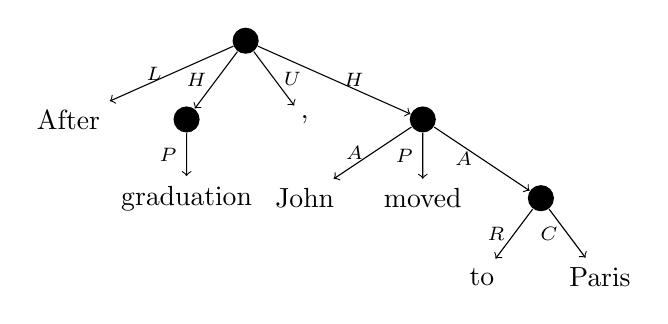
\begin{tikzpicture}[level distance=10mm, ->]
    \node (ROOT) [fill=black, circle] {}
      child {node (After) {After} edge from parent node[left] {\scriptsize $L$}}
      child {node (graduation) [fill=black, circle] {}
      {
        child {node {graduation} edge from parent node[left] {\scriptsize $P$}}
      } edge from parent node[left] {\scriptsize $H$} }
      child {node {,} edge from parent node[right] {\scriptsize $U$}}
      child {node (moved) [fill=black, circle] {}
      {
        child {node (John) {John} edge from parent node[left] {\scriptsize $A$}}
        child {node {moved} edge from parent node[left] {\scriptsize $P$}}
        child {node [fill=black, circle] {}
        {
          child {node {to} edge from parent node[left] {\scriptsize $R$}}
          child {node {Paris} edge from parent node[left] {\scriptsize $C$}}
        } edge from parent node[left] {\scriptsize $A$} }
      } edge from parent node[right] {\scriptsize $H$} }
      ;
  \end{tikzpicture}
}
\scalebox{.9}{
	\begin{dependency}[theme = simple]
	\begin{deptext}[column sep=.7em,ampersand replacement=\^]
	After \^ graduation \^ , \^ John \^ moved \^ to \^ Paris \\
	\end{deptext}
	\depedge{2}{1}{L}
	\depedge{2}{3}{U}
	\depedge{5}{4}{A}
	\depedge{2}{5}{H}
	\depedge{7}{6}{R}
	\depedge{5}{7}{A}
	\end{dependency}
  }
  \caption{Tree approximation for the sentence in \figref{fig:graduation} (top),
  and bilexical tree approximation for the same sentence (bottom).
  These are identical to the original graphs,
  apart from the removal of remote edges.}
  \label{fig:tree_example}
\end{figure}

\paragraph{Comparison to tree parsers.}
For completeness,
we also perform a \textit{tree approximation} experiment, converting UCCA to (bilexical) trees
and evaluating constituency and dependency tree parsers on them
(see examples in \figref{fig:tree_example}).
Our approach is similar
to the tree approximation approach used for dependency graph parsing
\cite{agic2015semantic,fernandez2015parsing},
where dependency graphs were converted into dependency trees
and then parsed by dependency tree parsers.
In our setting, the conversion to trees consists simply of removing remote edges from the 
graph, and then to bilexical trees by applying the same procedure as for bilexical graphs.

\paragraph{Baseline parsers.}
We evaluate two bilexical graph semantic dependency parsers:
DAGParser \cite{ribeyre-villemontedelaclergerie-seddah:2014:SemEval}, the leading 
transition-based parser in SemEval 2014 \cite{oepen2014semeval} and
TurboParser \cite{almeida-martins:2015:SemEval},
a graph-based parser from SemEval 2015 
\cite{oepen2015semeval};
\textsc{uparse} \cite{maier-lichte:2016:DiscoNLP},
a transition-based constituency parser supporting discontinuous constituents;
and two bilexical tree parsers:
MaltParser \cite{nivre2007maltparser},\footnote{For
MaltParser we use the \textsc{ArcEager} transition set and SVM classifier.
Other configurations yielded lower scores.}
and the stack LSTM-based parser of
\citet[henceforce ``LSTM Parser'']{dyer2015transition}.
Default settings are used in all cases.
DAGParser and \textsc{uparse} use beam search by default, with a beam size of 5 and 4
respectively. The other parsers are greedy.



%%%%%%%%%%%%%%%%%%%%%%%%%%%%%%%%%%%%%%%%%%%%%%%%%%%%%%%%%%%%%%%
\section{Results}\label{sec:results}

\tabref{table:results} presents our main experimental results, as well as
upper bounds for the baseline parsers,
reflecting the error resulting from the conversion.

DAGParser and \textsc{uparse} are most directly comparable to
\parser{Sparse}, as they also use a perceptron classifier with sparse features.
\parser{Sparse} considerably outperforms both, where
DAGParser does not predict any remote edges in the out-of-domain setting.
TurboParser fares worse in this comparison, despite somewhat better results on
remote edges.
The LSTM parser of \citet{dyer2015transition} obtains the highest primary F-score
among the baseline parsers, with a considerable margin.
It obtains 9.7\% F-score higher than MaltParser,
despite being limited by the same approximation error upper bound,
and using a similar transition set.
The performance difference between them should therefore be attributed to the classification model.

Using a feedforward NN and embedding features,
\parser{MLP} obtains higher scores than \parser{Sparse},
but is outperformed by the LSTM parser on primary edges.
However, using better input encoding,
\parser{BiLSTM} obtains substantially higher scores than \parser{MLP}
and all other parsers, on both primary and remote edges,
both in the in-domain and out-of-domain settings.
Its performance in absolute terms, of 73.5\% F-score on primary edges,
is encouraging in light of
UCCA's inter-annotator agreement of 80--85\%
F-score on them \cite{abend2013universal}.

The parsers resulting from tree approximation are unable to recover any remote edges,
as these are removed in the conversion.\footnote{We
also experimented with a simpler version of \parser{} lacking
\textsc{Remote} transitions, obtaining an increase of up to 2 labeled F-score
points on primary edges, at the cost of not being able to predict remote edges.}
The bilexical DAG parsers are also quite limited in this respect,
due to a conversion error upper bound of 58.3\%.
However, this upper bound cannot in itself account for the bilexical DAG parsers'
poor performance on remote edges, which is an order of magnitude lower than that
of \parser{BiLSTM}.






%%%%%%%%%%%%%%%%%%%%%%%%%%%%%%%%%%%%%%%%%%%%%%%%%%%%%%%%%%%%%%%

\section{Related Work}\label{sec:related_work}

While earlier work on anchored\footnote{By {\it anchored} we mean that the semantic representation
directly corresponds to the words and phrases of the text.}
semantic parsing has mostly concentrated on shallow semantic analysis,
focusing on semantic role labeling of verbal argument structures,
the focus has recently shifted to parsing of more elaborate representations that account
for a wider range of phenomena.

\paragraph{Grammar-Based Parsing.}
Linguistically expressive grammars such as HPSG \cite{PandS:94}, CCG \cite{Steedman:00} and TAG \cite{Joshi:97}
provide a theory of the syntax-semantics interface, and have been used as a basis for semantic parsers
by defining compositional semantics on top of them \cite[among others]{Flic:00,bos2005towards}.
Depending on the grammar and the implementation, such semantic parsers can support
some or all of the structural properties UCCA exhibits.
Nevertheless, this line of work differs from our grammarless approach in two important ways.
First, the \textit{representations} are different. UCCA does not attempt to model
the syntax-semantics interface and is thus less coupled with syntax.
Second, while grammar-based \textit{parsers} explicitly model syntax, grammarless
approaches, as presented here, directly model the relation between
tokens and semantic structures.

\paragraph{Broad-Coverage Semantic Parsing.}
Most closely related to this work is Broad-Coverage Semantic Dependency Parsing (SDP),
addressed in two SemEval tasks \cite{oepen2014semeval,oepen2015semeval}.
Like UCCA parsing, SDP addresses a wide range of semantic phenomena,
and supports discontinuous units and reentrancy.
However, SDP uses bilexical dependencies, disallowing non-terminal nodes,
useful for representing structures that have no clear head, such as coordination
\cite{Ivanova2012who}. It also differs from UCCA in the type
of distinctions it makes, which are more tightly coupled with syntactic considerations,
where UCCA aims to capture purely semantic cross-linguistically applicable notions.
For instance, the ``poss'' label in the DM target representation is used to
annotate syntactic possessive constructions, regardless of whether they correspond to
semantic ownership (e.g., ``John's dog'') or other semantic relations,
such as marking an argument of a nominal predicate (e.g., ``John's kick'').

Recent interest in SDP has yielded numerous works on graph parsing
\cite{ribeyre-villemontedelaclergerie-seddah:2014:SemEval,thomson-EtAl:2014:SemEval,almeida-martins:2015:SemEval,du-EtAl:2015:SemEval}, including
tree approximation \cite{agic-koller:2014:SemEval,schluter-EtAl:2014:SemEval}
and joint syntactic/semantic parsing
\cite{henderson2013multilingual,swayamdipta-EtAl:2016:CoNLL}.

\paragraph{Abstract Meaning Representation.}
Another line of work addresses parsing into AMRs
\cite{flanigan2014discriminative,vanderwende2015amr,pust2015parsing,artzi2015broad},
which, like UCCA, abstract away from syntactic distinctions
and represent meaning directly, using OntoNotes predicates \cite{weischedel2013ontonotes}.
Events in AMR may also be evoked by non-verbal predicates, including possessive constructions.
Unlike in UCCA, the alignment between AMR concepts and the text is not explicitly marked.
While sharing much of this work's motivation, not anchoring the representation in the text
complicates the parsing task, as it requires
the alignment to be automatically (and imprecisely) detected.
Indeed, despite considerable technical effort
\cite{flanigan2014discriminative,pourdamghani2014aligning,werling2015robust},
concept identification is only about 80\%--90\% accurate.
Furthermore, anchoring allows breaking down sentences into semantically meaningful sub-spans,
which is useful for many applications \cite{fernandez2015parsing,birch2016hume}.

Several transition-based AMR parsers have been proposed:
CAMR assumes syntactically parsed input,
processing dependency trees into AMR
\cite{wang-xue-pradhan:2015:ACL-IJCNLP,wang2015transition,wang-EtAl:2016:SemEval,goodman2016noise}.
In contrast,
the parser of \citet{damonte-17}
operates on the input tokens, but still requires concept identification, using
a simple heuristic selecting the most frequent graph for each token, and
\citet{zhou2016amr} perform concept identification and parsing jointly.
\parser{} does not require separately aligning the input tokens to the graph,
processing them directly instead,
and creating non-terminal units as part of the parsing process.
Furthermore, the transition sets used by the AMR parsers mentioned above
handle only a subset of reentrancies and discontinuities
(for example, \citet{damonte-17} pop the dependent in LArc transitions).
They are thus limited to a sub-class of AMRs in particular,
and of graphs that may be used in semantic parsing in general.
\parser{}'s transition set, on the other hand, allows general DAG parsing.



%%%%%%%%%%%%%%%%%%%%%%%%%%%%%%%%%%%%%%%%%%%%%%%%%%%%%%%%%%%%%%%
\section{Conclusion}\label{sec:conclusion}

We present \parser{}, the first parser for UCCA.
Evaluated in in-domain and out-of-domain settings, we show that coupled with a
NN classifier and BiLSTM feature extractor,
it accurately predicts UCCA graphs from text, outperforming a variety of
strong baselines by a margin.
Especially striking is the contribution of the LSTM-based feature representation,
unprecedented in syntactic dependency parsing \cite{andor2016globally}:
we speculate that semantic parsing inherently requires stronger models
to generalize across surface structures.
Despite the recent diversity of semantic parsing work,
the effectiveness of different approaches for
structurally and semantically different schemes is not well-understood
\cite{kuhlmann2016towards}.
Our contribution to this literature is a general grammarless parser
that supports multiple parents, discontinuous units and non-terminal nodes.

Future work will explore different target
representations and conversion procedures \cite{kong-15},
to compare different representations, suggesting ways for a data-driven design of semantic annotation.
A parser for UCCA will enable using the framework for new tasks,
in addition to existing applications such as machine translation
evaluation \cite{birch2016hume}.
We believe UCCA's merits in providing a cross-linguistically applicable,
broad-coverage annotation will support ongoing efforts to incorporate deeper
semantic structures into various applications,
such as sentence simplification \cite{narayan2014hybrid} and summarization \cite{liu2015toward}.

\bibliography{references}
\bibliographystyle{acl_natbib}

\end{document}
